%
% ---------------------------------------------------
%
% Proyecto Final de Carrera: EMIR
% Autor: Pedro Hernández Martín <alu3679@etsii.ull.es>
% Capítulo: Estado del arte
% Fichero: Cap2_estado_del_arte.tex
%
% ----------------------------------------------------
%

\chapter{Resultados} \label{chap:resultados}
En este capítulo se presentan los resultados obtenidos con diversas
distribuciones de objetos, tanto generadas de forma sintética y ex-profeso para
comprobar la aplicación, como correspondientes a casos reales. Todos estos
ejemplos se incluyen en el directorio \texttt{ejemplos/} de la aplicación.

Los resultados se muestran en tablas que recogen el número de CSUs que
constituye la solución junto al tiempo (en minutos y segundos) que ha tardado en calcularse la misma,
dependiendo de las opciones que se utilicen en la ejecución. Las opciones se
muestran a la izquierda, por filas, mientras que el tipo de resultado se muestra
en la parte superior, en las columnas.

También se muestran pares de imágenes, correspondientes a la entrada y la salida
(sin especificación de ningún tipo de parámetros adicionales) del programa, para
facilitar la comprensión del ejemplo. La figura de la izquierda representa la
nube de objetos sobre la que el \CSUO{} va a buscar los apuntados, y la
figura de la derecha muestra el resultado obtenido. Se dibuja de un color
diferente cada apuntado para facilitar su diferenciación.

Para los cálculos se ha utilizado una máquina virtual con Ubuntu 12.04 LTS, dos
procesadores y 2 GB de memoria RAM, que corre bajo un Windows 7 nativo, con un
Intel i7 920 (2.67 GHz) y 6 GB de memoria RAM DDR3.

\section{Ejemplos sintéticos} \label{sec:sintetico}
Son ejemplos generados por el ``editor de mapas'' (\texttt{mapEditor}) para depurar la aplicación y
comprobar su comportamiento. Algunas de las distribuciones se generaron de forma
aleatoria, por lo que no hay manera de saber si los resultados son óptimos o
no. Otros ejemplos se han generado siguiendo un patrón concreto, para el que
conocemos de antemano la solución óptima. Para ello situamos en el espacio de
trabajo una CSU ``virtual'' sobre la que colocamos un cierto número de objetos
distribuidos de tal modo que sabemos que ajustan perfectamente con las barra de
esta CSU ``virtual''.
Si el \CSUO{} realiza correctamente su trabajo, colocará una CSU (apuntado) configurado
exactamente igual que la CSU ``virtual'' que ubicamos con el \texttt{mapEditor}.

\subsection {Ejemplo: \texttt{exacto.xml}}
Este ejemplo consiste en 55 objetos a observar distribuidos de forma que cada
uno de ellos ajuste perfectamente dentro de una barra de la CSU, siendo el
resultado óptimo un único apuntado. Al tratarse de un ejemplo creado con el ``editor de
mapas'' la distancia de cada punto es la necesaria para que el resultado no
varíe entre las diversas opciones que se permiten.

%%%%%%%%%%%%%%%%%%%%% Fig. %%%%%%%%%%%%%%%%%%%%%%%%%%%%%%%%%%%
%\begin{figure}[ht]
%\centering
%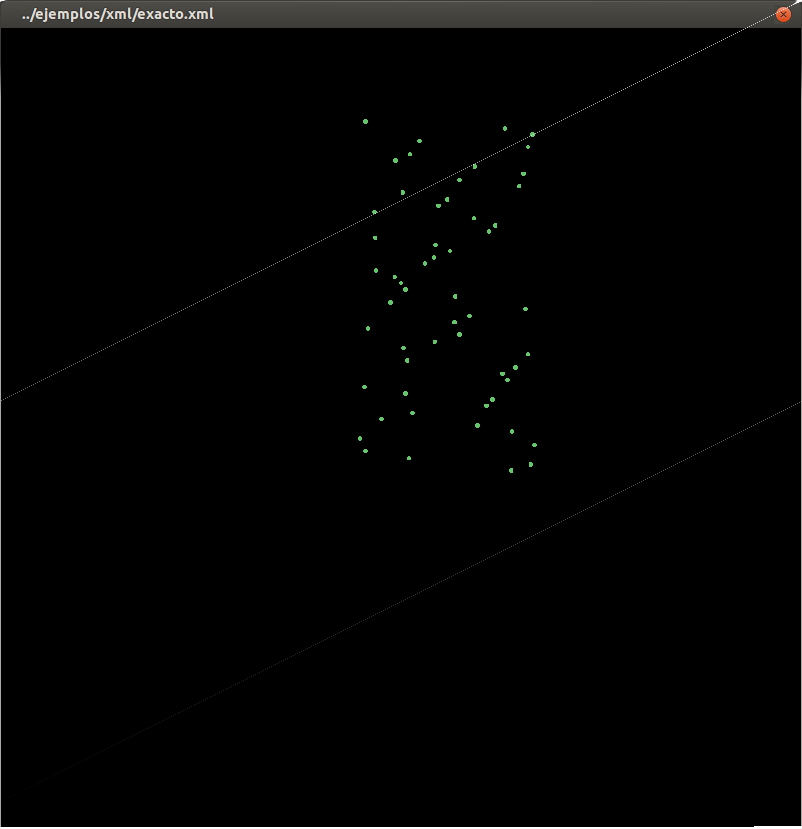
\includegraphics[height=7.5cm]{exacto-in} 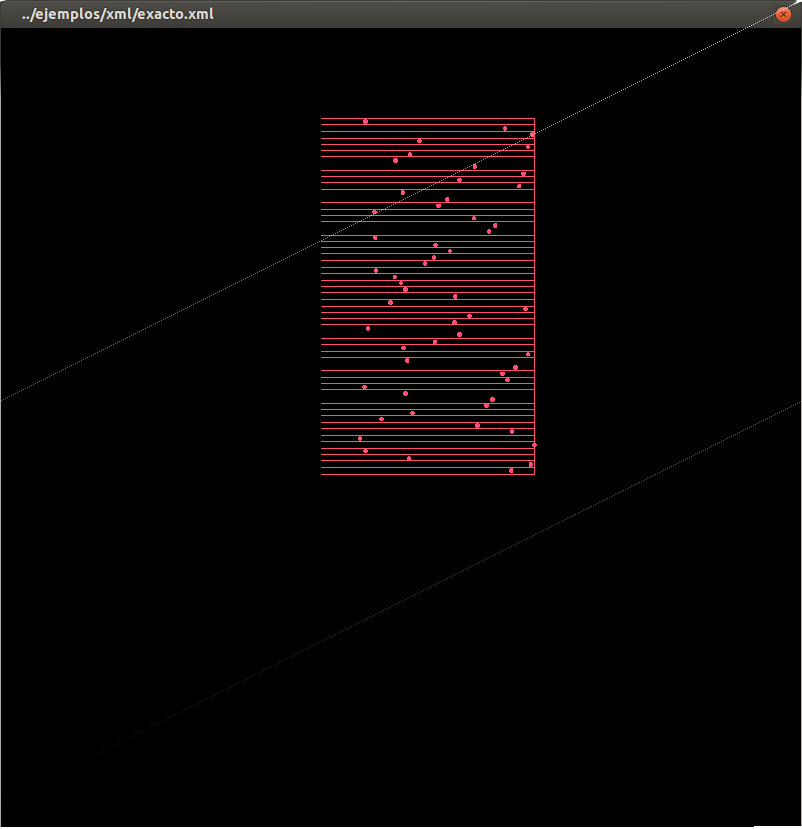
\includegraphics[height=7.5cm]{exacto-out}
%\caption{Ejemplo \texttt{exacto.xml}. 55 objetos que se ajustan perfectamente a una única CSU}
%\label{fig:3rodinia}
%\end{figure}
%%%%%%%%%%%%%%%%%%%%%%%%%%%%%%%%%%%%%%%%%%%%%%%%%%%%%%%%%%%%%

%%%%%%%%%%%%%%%%%%%% Fig. %%%%%%%%%%%%%%%%%%%%%%%%%%%%%%%%%%%
\begin{figure}[!htb]
\centering
\subfloat[Entrada]{
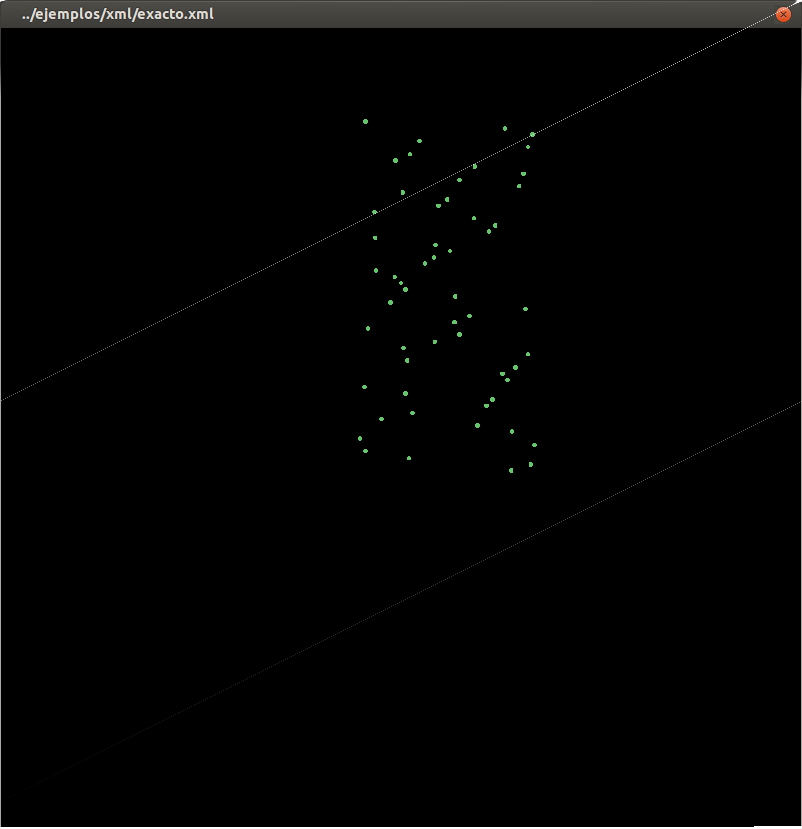
\includegraphics[width=0.5\linewidth]{exacto-in}
\label{fig:exacto-in}}
\subfloat[Salida del \CSUO{}]{ 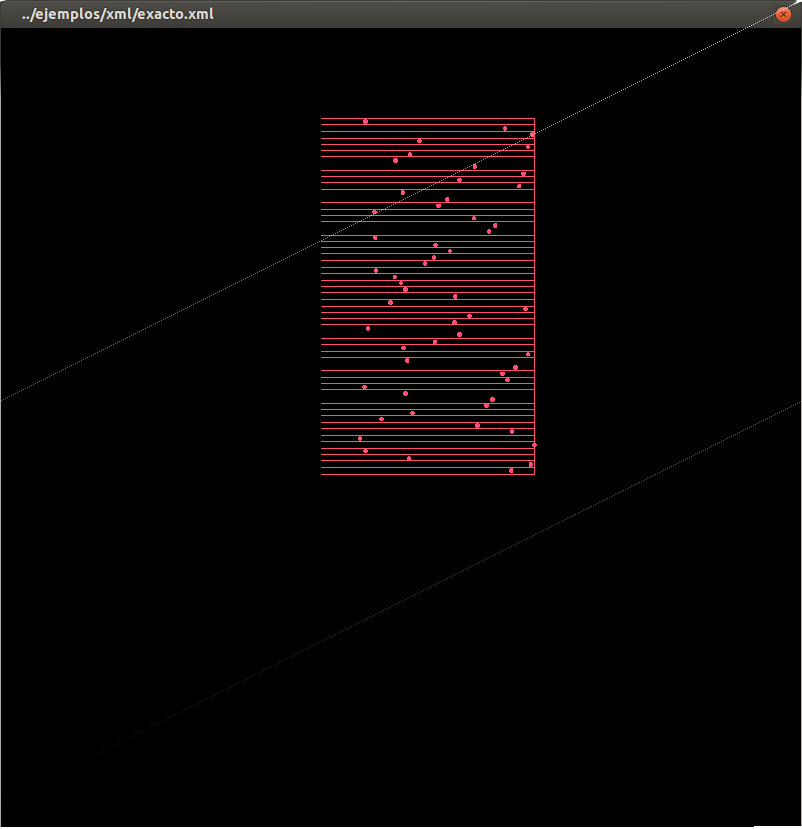
\includegraphics[width=0.5\linewidth]{exacto-out}
\label{fig:exacto-out}}
\caption{Ejemplo \texttt{exacto.xml}. 55 objetos que se ajustan perfectamente a una única CSU}
\end{figure}
%%%%%%%%%%%%%%%%%%%%%%%%%%%%%%%%%%%%%%%%%%%%%%%%%%%%%%%%%%%%%%
\begin{table*}[!ht]
\centering
\begin{tabular}{||l||c|c||}
\hline
\hline
RESULTADOS & Apuntados & Tiempo \\
\hline
\hline
Sin opciones & 1 & 1.02'' \\
\hline
Sin bordes & 1 & 0.76'' \\
\hline
Beam Switching & 1 & 0.72'' \\
\hline
Sin bordes + Beam S. & 1 & 0.89'' \\
\hline
\hline
\end{tabular}
\caption{Resultados del ejemplo \texttt{exacto.xml}}
\end{table*}

El resultado es justamente el esperado, por lo que comprobamos que la aplicación es capaz
de ajustar correctamente un apuntado de manera óptima para este tipo de instancias de entrada.

\subsection {Ejemplo: \texttt{4\_0solapes.xml}}
Este ejemplo consta de 220 objetos, que corresponden a cuatro apuntados
generados de forma que ninguno de ellos se solape con otro, con lo que el
resultado esperado son cuatro apuntados.

%%%%%%%%%%%%%%%%%%%% Fig. %%%%%%%%%%%%%%%%%%%%%%%%%%%%%%%%%%%
\begin{figure}[!htb]
\centering
\subfloat[Entrada]{
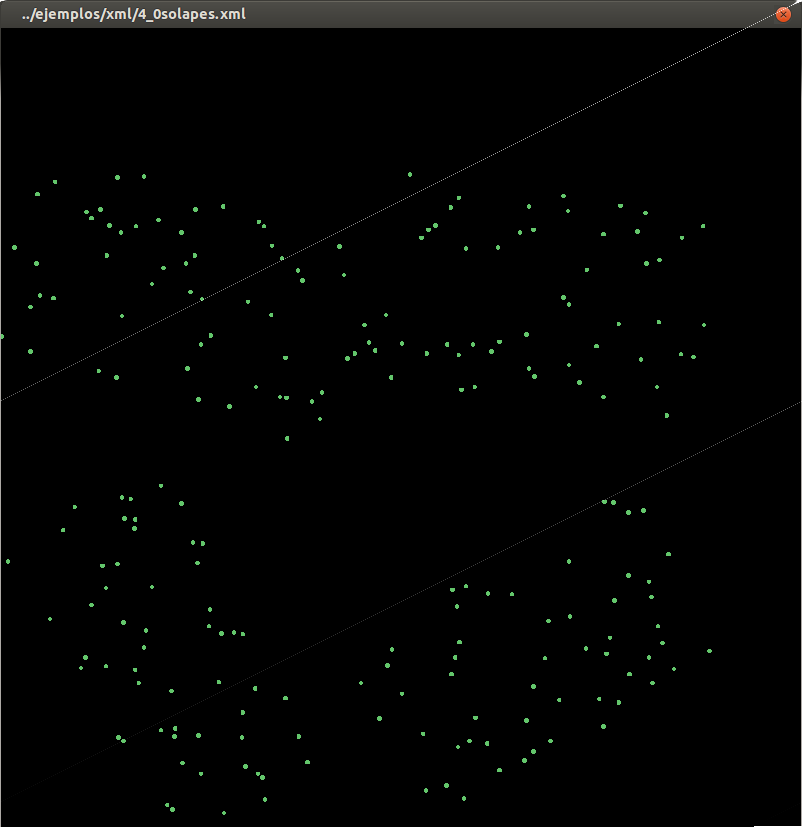
\includegraphics[width=0.5\linewidth]{4_0solapes-in}
\label{fig:4_0solapes-in}}
\subfloat[Salida del \CSUO{}]{
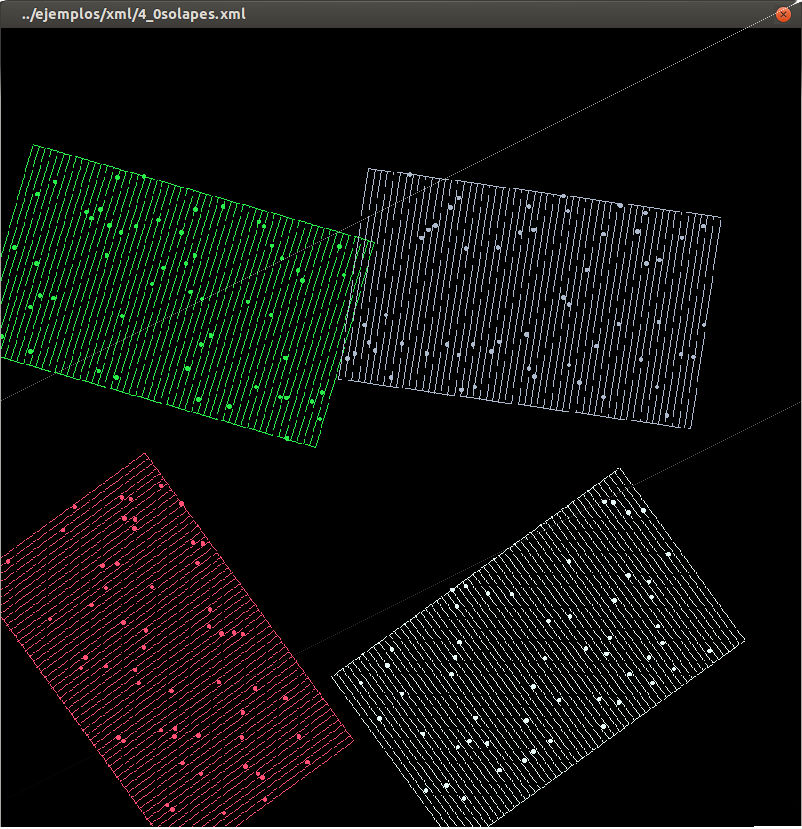
\includegraphics[width=0.5\linewidth]{4_0solapes-out}
\label{fig:4_0solapes-out}}
\caption{Ejemplo \texttt{4\_0solapes.xml}. 4 apuntados distanciados entre si}
\end{figure}
%%%%%%%%%%%%%%%%%%%%%%%%%%%%%%%%%%%%%%%%%%%%%%%%%%%%%%%%%%%%%%

\begin{table*}[!ht]
\centering
\begin{tabular}{||l||c|c||}
\hline
\hline
RESULTADOS & Apuntados & Tiempo \\
\hline
\hline
Sin opciones & 4 & 1.72'' \\
\hline
Sin bordes & 5& 2.97'' \\
\hline
Beam Switching & 4 & 3.09'' \\
\hline
Sin bordes + Beam S. & 4& 3.19'' \\
\hline
\hline
\end{tabular}
\caption{Resultados del ejemplo \texttt{4\_0solapes.xml}}
\label{tab:40solapes}
\end{table*}

Comprobamos en la Tabla \ref{tab:40solapes} que la aplicación se comporta tal y
como se pretende, salvo en uno de los casos. Este fallo de un apuntado de más se
debe a que en la solución inicial se crean 6 apuntados, cuya disposición
ocasiona que existan dos parejas de apuntados que solapan entre sí. Cuando el
método de reducción de colisiones evalúa estos solapes, consigue reducir aquella
pareja que se ha creado indebidamente, sin embargo la otra pareja corresponde
con un apuntado completo (con 55 objetos) y otro con un único objeto, de forma
que ambos apuntados son necesarios. Dada la disposición entre los apuntados
generados no se detectan colisiones a resolver, ocasionando el resultado
obtenido.
\subsection {Ejemplo: \texttt{4\_2solapes.xml}}
Este ejemplo tiene el mismo número de objetos que el anterior, 220, pero en este caso
se ha forzado a que dos apuntados solapen notablemente, para probar la calidad
del algoritmo que reduce las colisiones. Debido al alto grado de solape
existente se espera una solución relativamente mala.

%%%%%%%%%%%%%%%%%%%% Fig. %%%%%%%%%%%%%%%%%%%%%%%%%%%%%%%%%%%
\begin{figure}[!htb]
\centering
\subfloat[Entrada]{
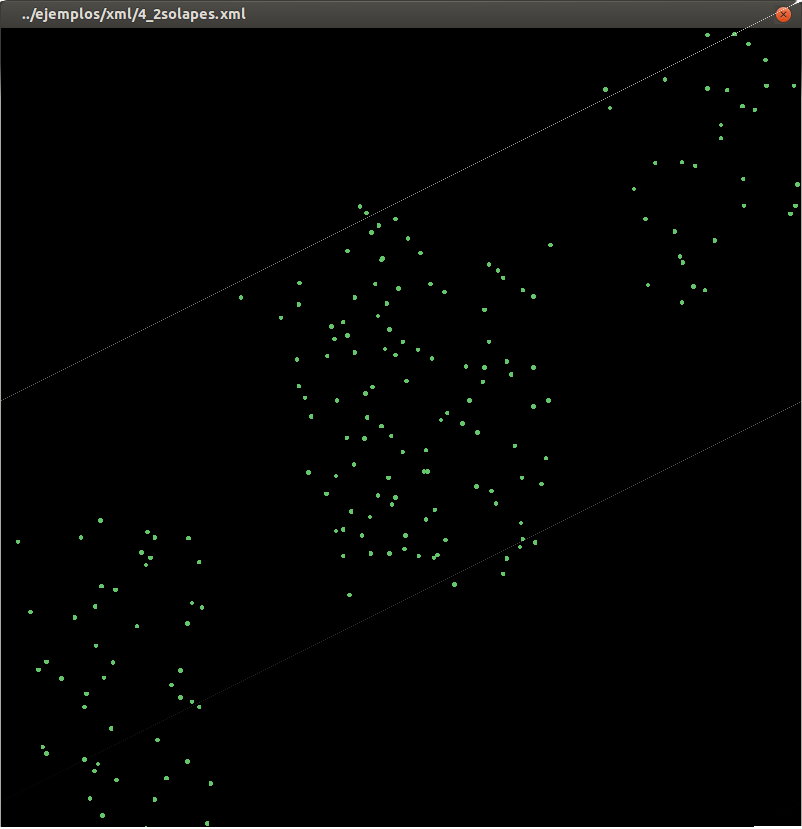
\includegraphics[width=0.5\linewidth]{4_2solapes-in}
\label{fig:4_2solapes-in}}
\subfloat[Salida del \CSUO{}]{
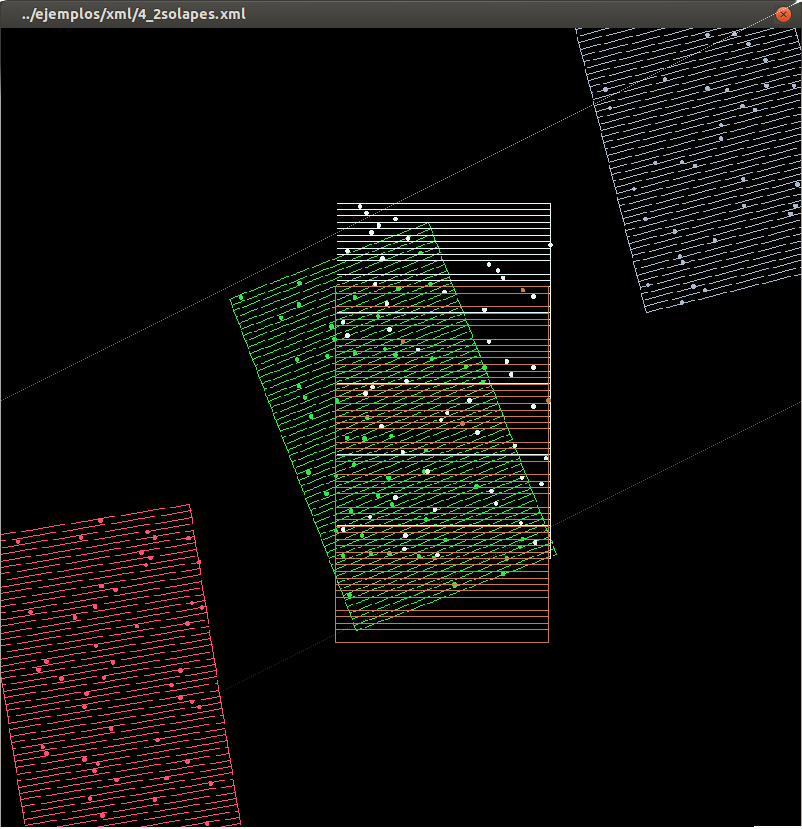
\includegraphics[width=0.5\linewidth]{4_2solapes-out}
\label{fig:4_2solapes-out}}
\caption{Ejemplo \texttt{4\_2solapes.xml}. Ejemplo de ``colisión'' de dos apuntados}
\end{figure}
%%%%%%%%%%%%%%%%%%%%%%%%%%%%%%%%%%%%%%%%%%%%%%%%%%%%%%%%%%%%%%

\begin{table*}[!ht]
\centering
\begin{tabular}{||l||c|c||}
\hline
\hline
RESULTADOS & Apuntados & Tiempo \\
\hline
\hline
Sin opciones & 5 & 4.26'' \\
\hline
Sin bordes & 5 & 3.64'' \\
\hline
Beam Switching & 5 & 4.29'' \\
\hline
Sin bordes + Beam S. & 5 & 3.67'' \\
\hline
\hline
\end{tabular}
\caption{Resultados del ejemplo \texttt{4\_2solapes.xml}}
\end{table*}

Pese al alto grado de solapamiento, la aplicación sólo ha introducido un
apuntado de más, por lo que se considera que el algoritmo ofrece resultados de razonable calidad
teniendo en cuenta el tiempo de ejecución.

\subsection {Ejemplo: \texttt{denso.xml}}
Este ejemplo no ha sido generado con la herramienta \texttt{mapEditor} sino que se
ha creado mediante una distribución aleatoria de los objetos, razón por la cual no podemos conocer a priori el
resultado óptimo. 
El ejemplo nos sirve para estudiar cómo se comporta la aplicación 
ante grandes nubes de objetos con una distribución espacial homogéneas. 
El ejemplo consta de 999 puntos.

%%%%%%%%%%%%%%%%%%%% Fig. %%%%%%%%%%%%%%%%%%%%%%%%%%%%%%%%%%%
\begin{figure}[!htb]
\centering
\subfloat[Entrada]{
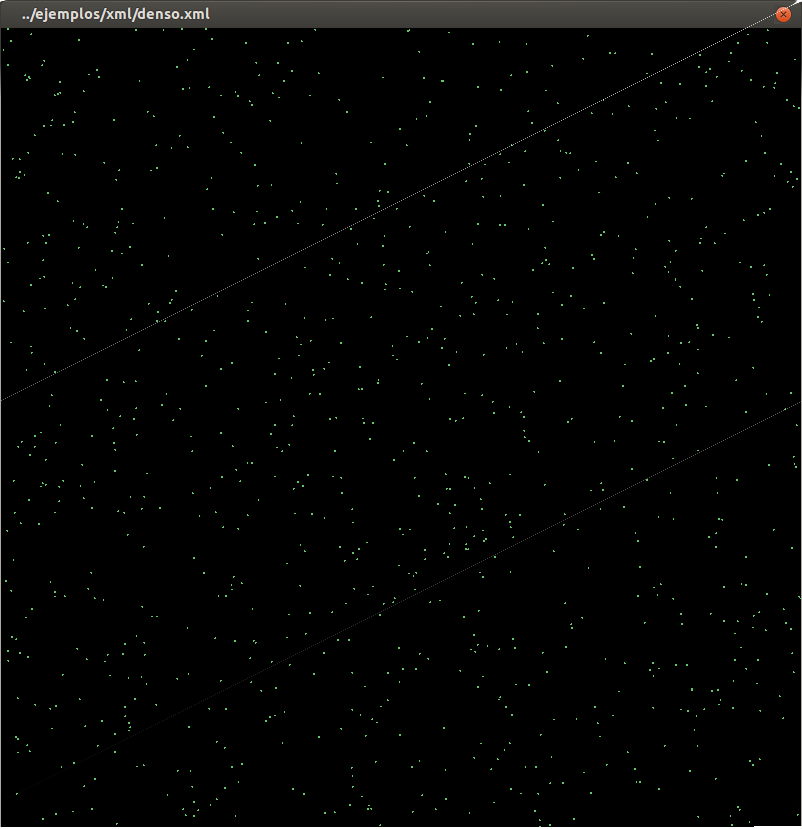
\includegraphics[width=0.5\linewidth]{denso-in}
\label{fig:denso-in}}
\subfloat[Salida del \CSUO{}]{
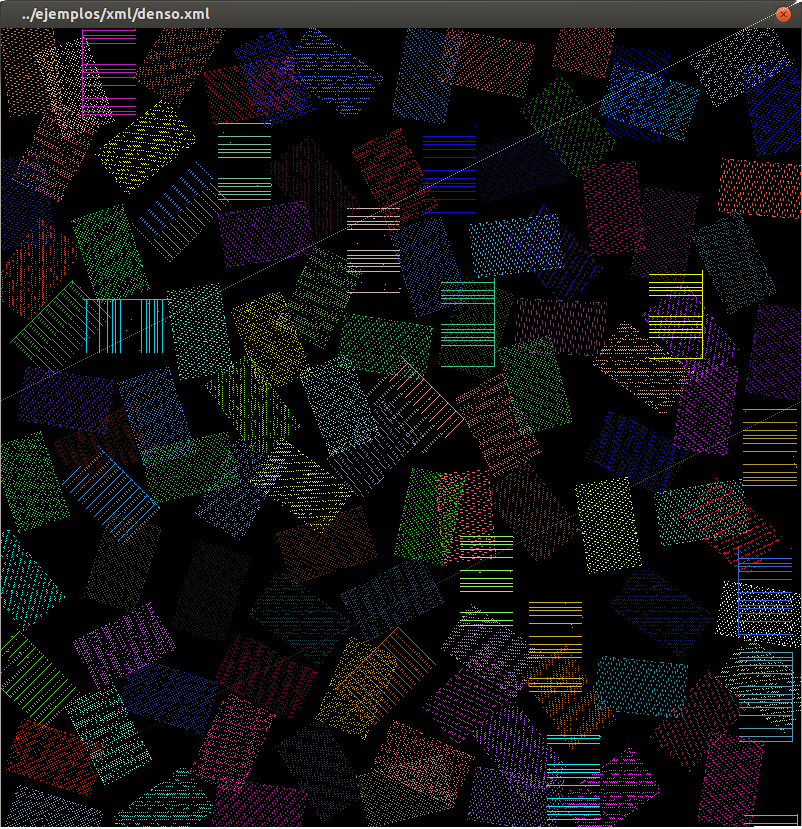
\includegraphics[width=0.5\linewidth]{denso-out}
\label{fig:denso-out}}
\caption{Ejemplo \texttt{denso.xml}. Gran número de objetos distribuidos homogéneamente}
\end{figure}
%%%%%%%%%%%%%%%%%%%%%%%%%%%%%%%%%%%%%%%%%%%%%%%%%%%%%%%%%%%%%%

\begin{table*}[!ht]
\centering
\begin{tabular}{||l||c|c||}
\hline
\hline
RESULTADOS & Apuntados & Tiempo \\
\hline
\hline
Sin opciones & 110 & 26.93'' \\
\hline
Sin bordes & 118 & 20.02'' \\
\hline
Beam Switching & 150 & 42.87'' \\
\hline
Sin bordes + Beam S. & 175 & 1' 1.78'' \\
\hline
\hline
\end{tabular}
\caption{Resultados del ejemplo \texttt{denso.xml}}
\label{tabla:denso}
\end{table*}

\subsection {Ejemplo: \texttt{denso2000.xml}}
Se trata del mismo ejemplo anterior, incrementando el número de objetos hasta 2000. 
Esta entrada se generó con el fin de evaluar el tiempo tarda el \CSUO{} en generar soluciones para ejemplos
relativamente grandes.

%%%%%%%%%%%%%%%%%%%% Fig. %%%%%%%%%%%%%%%%%%%%%%%%%%%%%%%%%%%
\begin{figure}[!htb]
\centering
\subfloat[Entrada]{
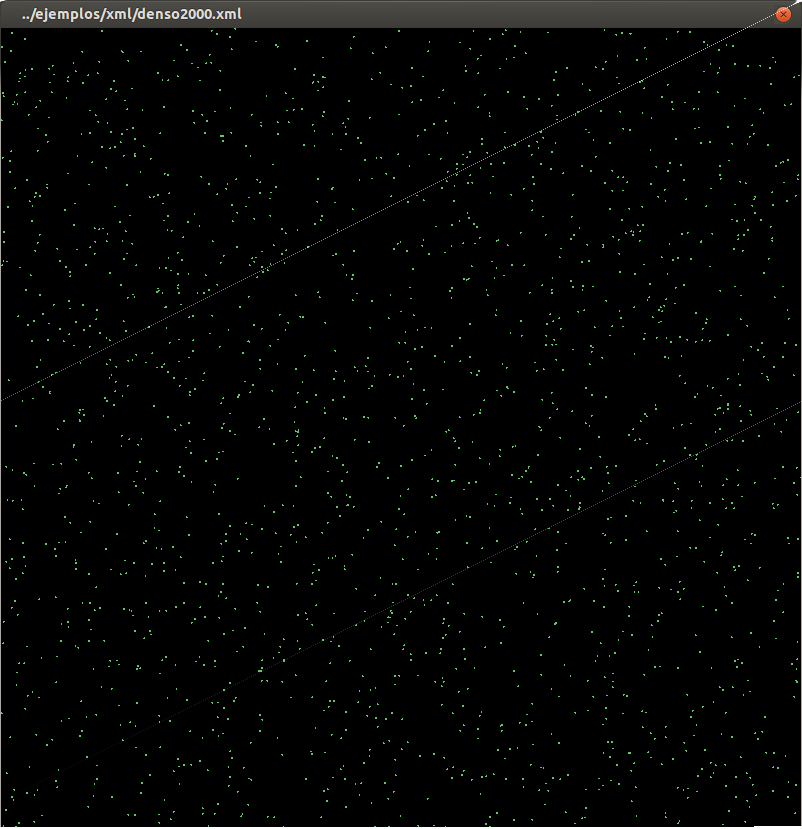
\includegraphics[width=0.5\linewidth]{denso2000-in}
\label{fig:denso2000-in}}
\subfloat[Salida del \CSUO{}]{
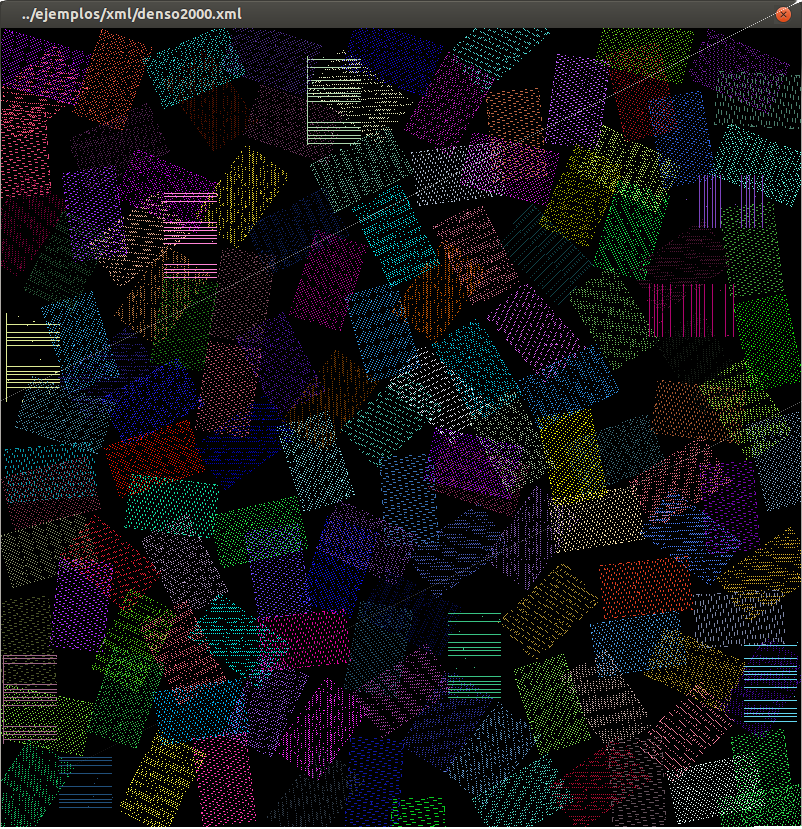
\includegraphics[width=0.5\linewidth]{denso2000-out}
\label{fig:denso2000-out}}
\caption{Ejemplo \texttt{denso2000.xml}. 2000 objetos generados aleatoriamente y distribuidos de forma homogénea}
\end{figure}
%%%%%%%%%%%%%%%%%%%%%%%%%%%%%%%%%%%%%%%%%%%%%%%%%%%%%%%%%%%%%%

\begin{table*}[!ht]
\centering
\begin{tabular}{||l||c|c||}
\hline
\hline
RESULTADOS & Apuntados & Tiempo \\
\hline
\hline
Sin opciones & 135 & 1' 42.69'' \\
\hline
Sin bordes & 152 & 2' 17.52'' \\
\hline
Beam Switching & 217 & 3' 44.53'' \\
\hline
Sin bordes + Beam S. & 296 & 3' 20.97'' \\
\hline
\hline
\end{tabular}
\caption{Resultados del ejemplo \texttt{denso2000.xml}}
\end{table*}

Si se comparan los resultados del ejemplo anterior (Tabla \ref{tabla:denso}) con
los de este caso, se comprueba que los tiempos no aumentan linealmente conforme
aumenta el tamaño del problema: se han duplicado los objetos pero los tiempos no
presentan esta proporcionalidad. 
% XXX <-- Ojo a esa afirmación: los tiempos a lo mejor no se doblan de forma exacta, pero no estoy seguro de lo que dices.
% Comentame algo al respecto.
Este efecto se debe a que el tiempo final no depende tanto del número de
puntos sino de cómo estos están distribuidos espacialmente. 
A mayor número de colisiones, mayor número de comprobaciones tendrá que hacer la aplicación.

\subsection {Ejemplo: \texttt{disperso.xml}}
Este ejemplo consta de 200 objetos repartidos aleatoriamente, de forma que no se
formen nubes de gran densidad, obteniendo así un caso en el que los objetos 
tienen una cierta distancia entre ellos. Es este caso el número de apuntados
debería ser cercano al número de objetos, puesto que con esta disposición es
poco probable encontrar grupos cercanos agrupables en una única CSU.

%%%%%%%%%%%%%%%%%%%% Fig. %%%%%%%%%%%%%%%%%%%%%%%%%%%%%%%%%%%
\begin{figure}[!htb]
\centering
\subfloat[Entrada]{
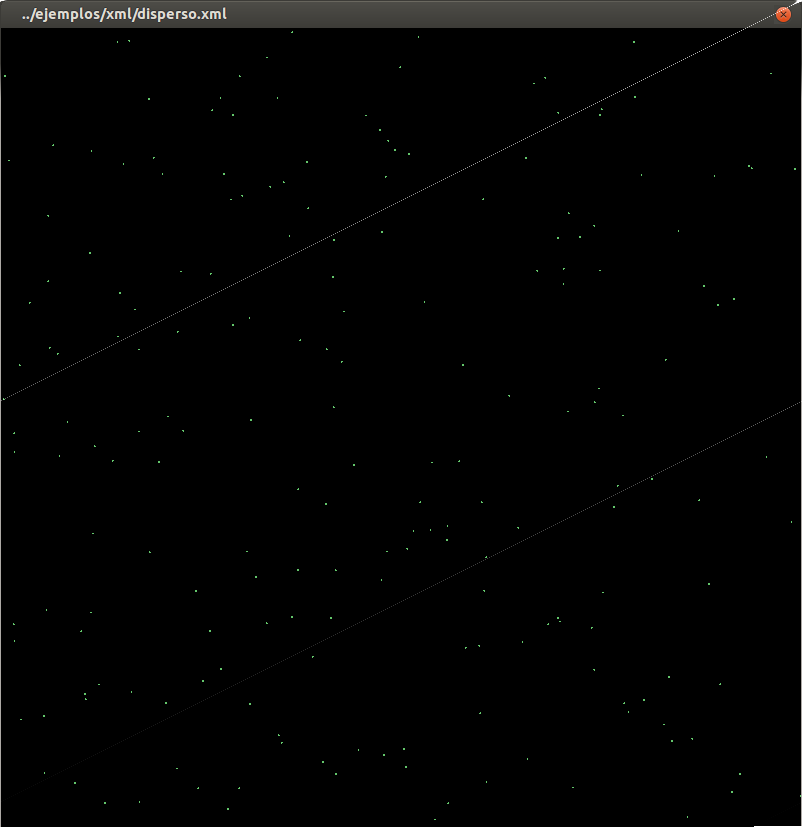
\includegraphics[width=0.5\linewidth]{disperso-in}
\label{fig:disperso-in}}
\subfloat[Salida del \CSUO{}]{
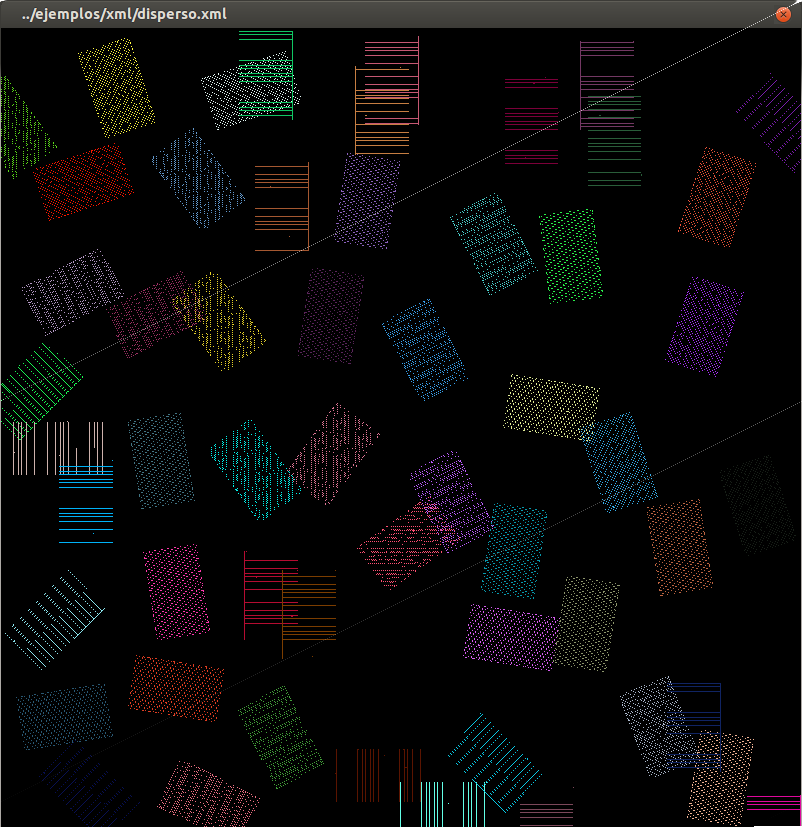
\includegraphics[width=0.5\linewidth]{disperso-out}
\label{fig:disperso-out}}
\caption{Ejemplo \texttt{disperso.xml}. 200 objetos distribuidos en un campo de un grado cuadrado}
\end{figure}
%%%%%%%%%%%%%%%%%%%%%%%%%%%%%%%%%%%%%%%%%%%%%%%%%%%%%%%%%%%%%%

\begin{table*}[!ht]
\centering
\begin{tabular}{||l||c|c||}
\hline
\hline
RESULTADOS & Apuntados & Tiempo \\
\hline
\hline
Sin opciones & 55 & 2.20'' \\
\hline
Sin bordes & 55& 2.16'' \\
\hline
Beam Switching & 61 & 2.66'' \\
\hline
Sin bordes + Beam S. & 67& 2.85'' \\
\hline
\hline
\end{tabular}
\caption{Resultados del ejemplo \texttt{disperso.xml}}
\end{table*}

El número de apuntados obtenido presenta una media de unos 4 objetos por
apuntado, significativamente inferior a su capacidad de 55 objetos, como cabe esperar 
de la baja densidad del ejemplo.

\subsection {Ejemplo: \texttt{clusters.xml}}
Para este ejemplo se han generado tres nubes de objetos separadas entre
si, cuyos objetos están dispuestos aleatoriamente, impidiendo conocer a priori
el resultado óptimo. El número total de objetos es de 146.
El objetivo de esta prueba era comprobar que la función
que reduce las colisiones no trataba apuntados o elementos que estuvieran
separados.
%%%%%%%%%%%%%%%%%%%% Fig. %%%%%%%%%%%%%%%%%%%%%%%%%%%%%%%%%%%
\begin{figure}[!htb]
\centering
\subfloat[Entrada]{
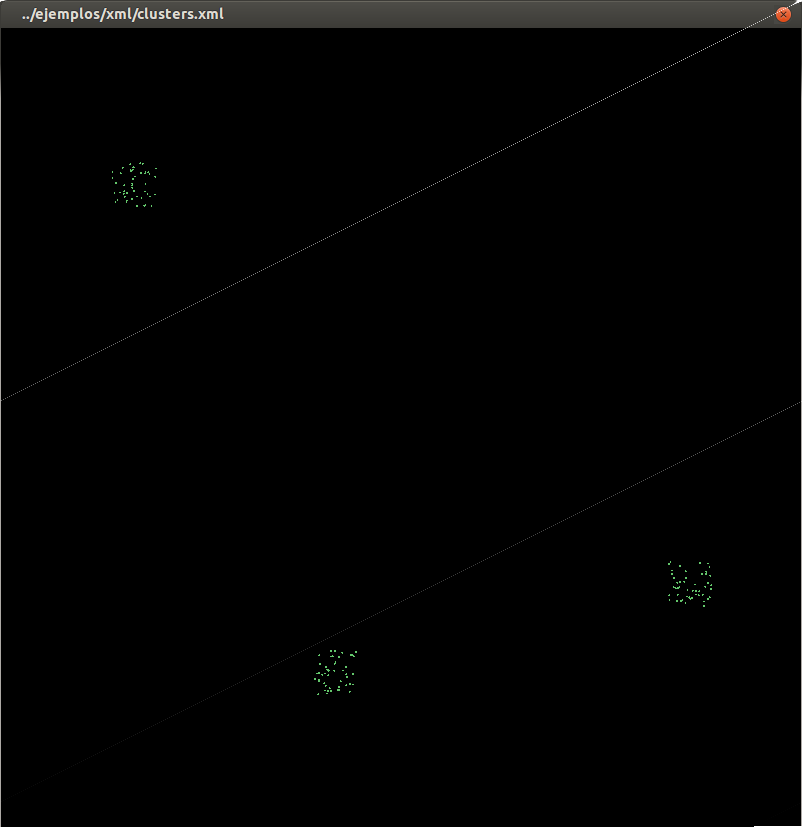
\includegraphics[width=0.5\linewidth]{clusters-in} 
\label{fig:clusters-in}}
\subfloat[Salida del \CSUO{}]{
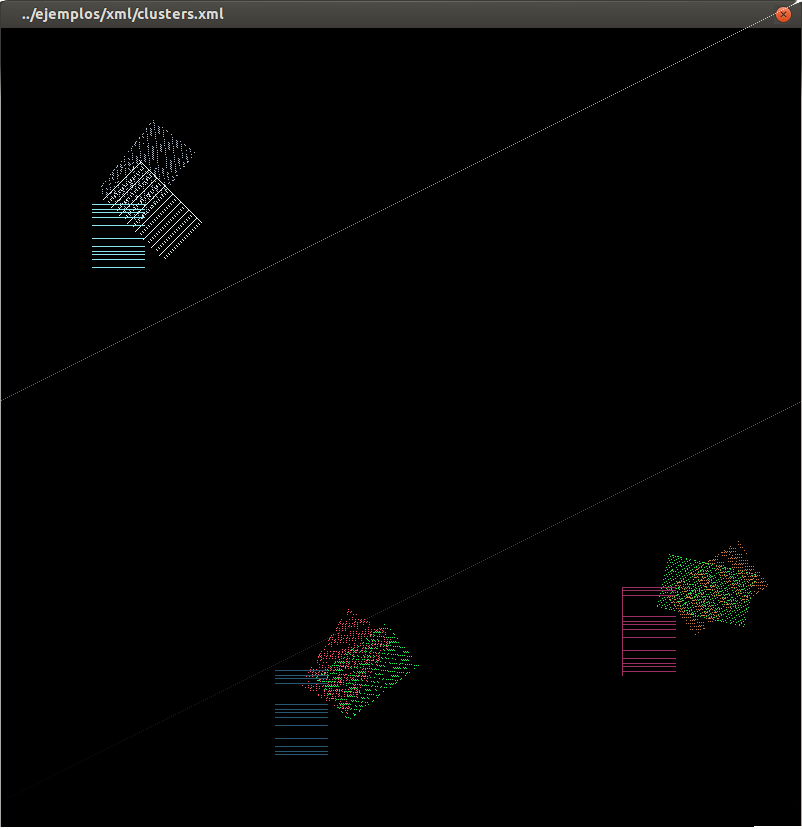
\includegraphics[width=0.5\linewidth]{clusters-out}
\label{fig:clusters-out}}
\caption{Ejemplo \texttt{clusters.xml}. Pequeño grupo de objetos agrupados en tres clústers independientes}
\end{figure}
%%%%%%%%%%%%%%%%%%%%%%%%%%%%%%%%%%%%%%%%%%%%%%%%%%%%%%%%%%%%%%

\begin{table*}[!ht]
\centering
\begin{tabular}{||l||c|c||}
\hline
\hline
RESULTADOS & Apuntados & Tiempo \\
\hline
\hline
Sin opciones & 9 & 2.79'' \\
\hline
Sin bordes &9 & 2.69'' \\
\hline
Beam Switching & 12 & 5.18'' \\
\hline
Sin bordes + Beam S. & 15& 5.43'' \\
\hline
\hline
\end{tabular}
\caption{Resultados del ejemplo \texttt{clusters.xml}}
\end{table*}

\section{Ejemplos reales}
En esta sección se presentan ejemplos que no han sido generados de manera
sintética como los anteriores, sino que han sido aportados por el responsable del
proyecto EMIR para comprobar el funcionamiento de la aplicación ante distribuciones de
objetos reales (o al menos más realistas).

\subsection {Ejemplo: \texttt{real1.xml}}
Este ejemplo ha sido clave para comprobar la calidad de los resultados
obtenidos, puesto que se conoce a priori el número óptimo de apuntados
necesarios para resolverlo, siendo este valor de 65 apuntados. El ejemplo
consta de un conjunto de aproximadamente 2000 objetos dispersos en un campo de un
grado cuadrado, esto es, 3600$\times$3600 arcosegundos.

%%%%%%%%%%%%%%%%%%%% Fig. %%%%%%%%%%%%%%%%%%%%%%%%%%%%%%%%%%%
\begin{figure}[!htb]
\centering
\subfloat[Entrada]{
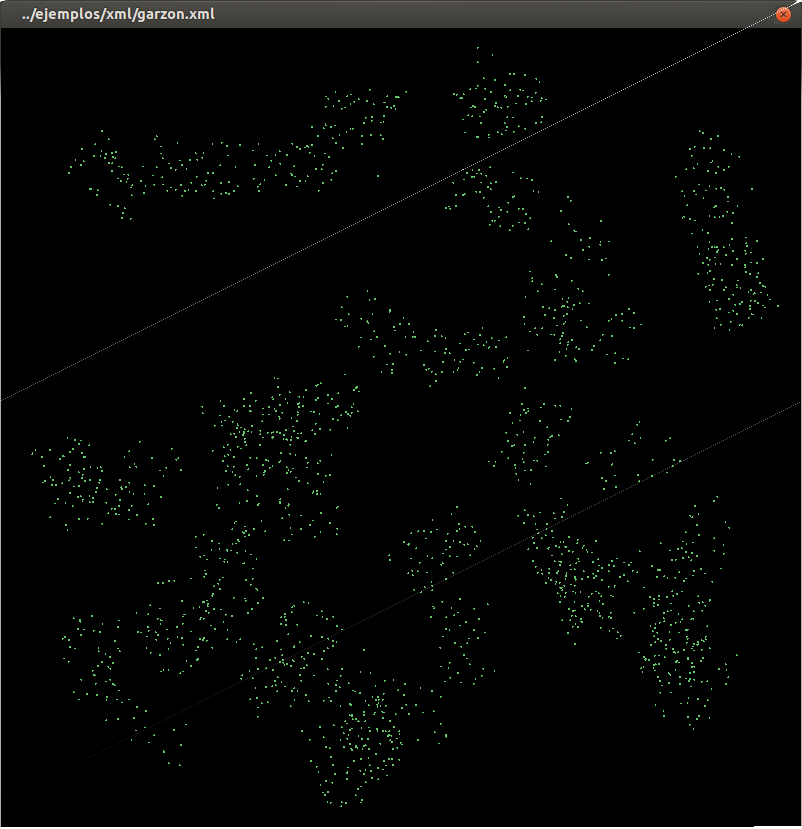
\includegraphics[width=0.5\linewidth]{real1-in} 
\label{fig:real1-in}}
\subfloat[Salida del \CSUO{}]{
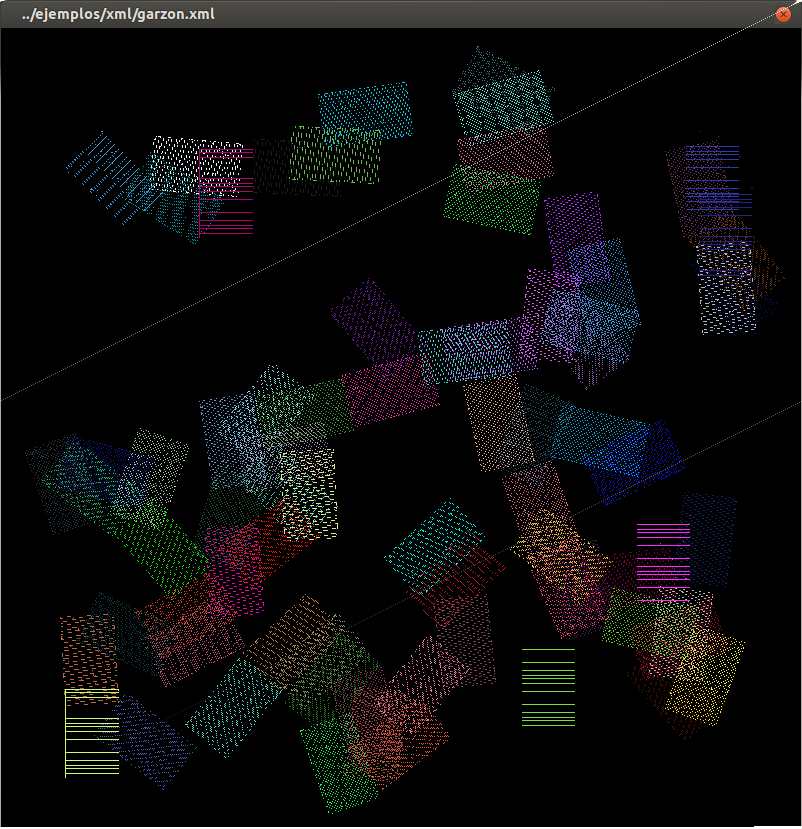
\includegraphics[width=0.5\linewidth]{real1-out}
\label{fig:real1-out}}
\caption{Ejemplo \texttt{real1.xml}. Caso real de 2000 objetos que siguen una distribución uniforme}
\end{figure}
%%%%%%%%%%%%%%%%%%%%%%%%%%%%%%%%%%%%%%%%%%%%%%%%%%%%%%%%%%%%%%

\begin{table*}[!ht]
\centering
\begin{tabular}{||l||c|c||}
\hline
\hline
RESULTADOS & Apuntados & Tiempo \\
\hline
\hline
Sin opciones & 75 & 2' 53.69'' \\
\hline
Sin bordes &91 & 2' 3.21'' \\
\hline
Beam Switching & 142 & 4' 1.28'' \\
\hline
Sin bordes + Beam S. & 181& 5' 33.68'' \\
\hline
\hline
\end{tabular}
\caption{Resultados del ejemplo \texttt{real1.xml}}
\end{table*}

El resultado obtenido se acerca al óptimo, dando 10 apuntados más de
los deseados. Puede verse como una extensión del problema \texttt{4\_2solapes}
analizado anteriormente. Al existir mucho solape entre apuntados, el algoritmo
tarda al intentar reducirlos, aunque no siempre toma la mejor elección
posible de objetos, situando en un apuntado un elemento que iría mejor en otro.
No obstante el resultado es razonablemente bueno, confirmando nuestra hipótesis sobre
el buen funcionamiento del algoritmo.

\subsection {Ejemplo: \texttt{real2.xml}}
El ejemplo que sigue a continuación tiene una cantidad de objetos mucho menor a
la que podríamos esperar de un caso real, puesto que consta solamente de 297
objetos. Se desconoce su resultado óptimo.

%%%%%%%%%%%%%%%%%%%% Fig. %%%%%%%%%%%%%%%%%%%%%%%%%%%%%%%%%%%
\begin{figure}[!htb]
\centering
\subfloat[Entrada]{
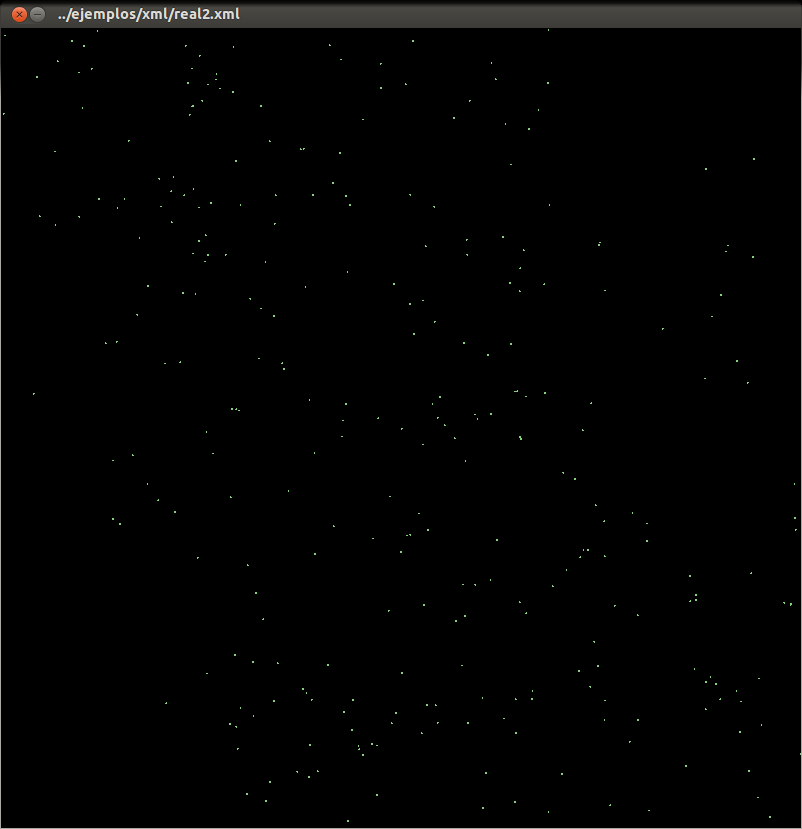
\includegraphics[width=0.5\linewidth]{real2-in} 
\label{fig:real2-in}}
\subfloat[Salida del \CSUO{}]{
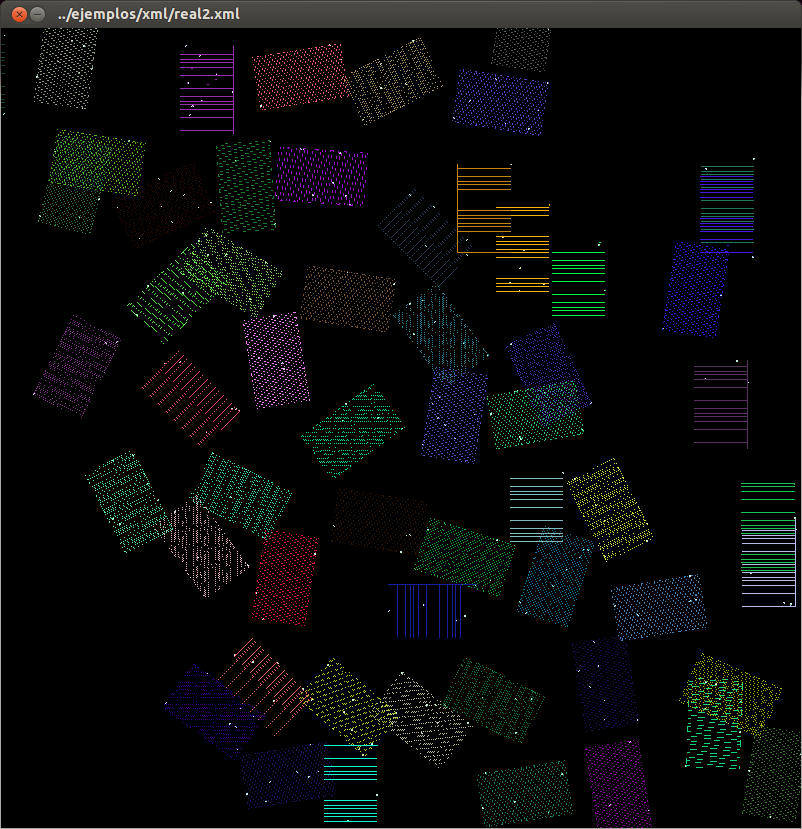
\includegraphics[width=0.5\linewidth]{real2-out}
\label{fig:real2-out}}
\caption{Ejemplo \texttt{real2.xml}. Aproximadamente 300 objetos reales}
\end{figure}
%%%%%%%%%%%%%%%%%%%%%%%%%%%%%%%%%%%%%%%%%%%%%%%%%%%%%%%%%%%%%%

\begin{table*}[!ht]
\centering
\begin{tabular}{||l||c|c||}
\hline
\hline
RESULTADOS & Apuntados & Tiempo \\
\hline
\hline
Sin opciones & 57 & 3.85'' \\
\hline
Sin bordes & 56 & 3.91'' \\
\hline
Beam Switching & 70 & 6.24'' \\
\hline
Sin bordes + Beam S. & 79& 7.08'' \\
\hline
\hline
\end{tabular}
\caption{Resultados del ejemplo \texttt{real2.xml}}
\end{table*}

En el segundo caso, en el cual se ejecuta la opción de quitar un mínimo espacio
a los bordes, obtenemos un mejor resultado. Esto se debe, como podemos intuir,
a que al obligar que los objetos se sitúen en un espacio más reducido, es
posible que la forma en la que se coloquen evite que un elemento que
antiguamente nos producía un mal intercambio de puntos entre a formar parte del
apuntado.

\subsection {Ejemplo: \texttt{cluster1.xml}}
El siguiente ejemplo es un caso real con 1398 objetos situados formando un
círculo alrededor del centro de un espacio de 4187 arcosegundos de ancho por
4183 arcosegundos de alto.

%%%%%%%%%%%%%%%%%%%% Fig. %%%%%%%%%%%%%%%%%%%%%%%%%%%%%%%%%%%
\begin{figure}[!htb]
\centering
\subfloat[Entrada]{
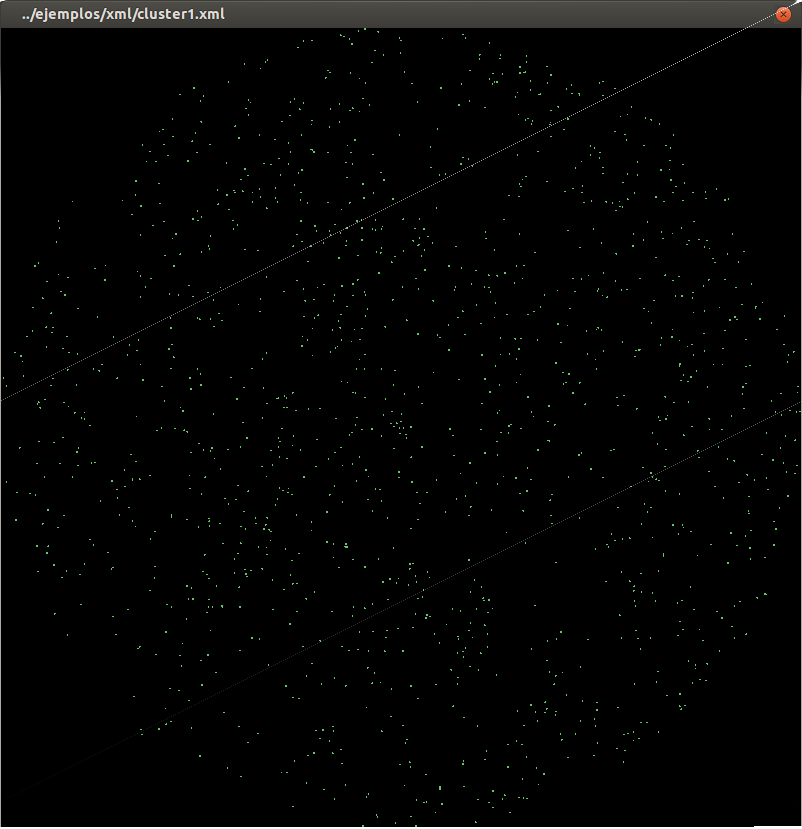
\includegraphics[width=0.5\linewidth]{cluster1-in} 
\label{fig:cluster1-in}}
\subfloat[Salida del \CSUO{}]{
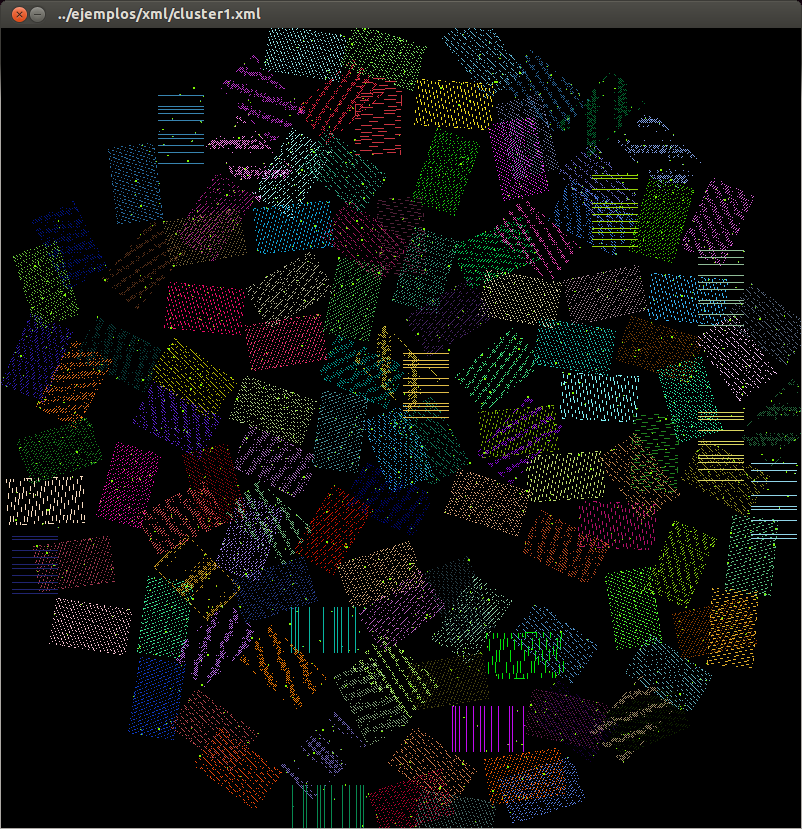
\includegraphics[width=0.5\linewidth]{cluster1-out}
\label{fig:cluster1-out}}
\caption{Ejemplo \texttt{cluster1.xml}. Caso real cuyos objetos muestran una distribución concéntrica.}
\end{figure}
%%%%%%%%%%%%%%%%%%%%%%%%%%%%%%%%%%%%%%%%%%%%%%%%%%%%%%%%%%%%%%

\begin{table*}[!ht]
\centering
\begin{tabular}{||l||c|c||}
\hline
\hline
RESULTADOS & Apuntados & Tiempo \\
\hline
\hline
Sin opciones & 123 & 45.04'' \\
\hline
Sin bordes &138 & 45.05'' \\
\hline
Beam Switching & 180 & 1' 29.35'' \\
\hline
Sin bordes + Beam S. & 218 & 1' 59.17'' \\
\hline
\hline
\end{tabular}
\caption{Resultados del ejemplo \texttt{cluster1.xml}}
\end{table*}

\subsection {Ejemplo: \texttt{cluster2.xml}}
Este caso es similar al anterior, consta de 1842 elementos, aproximadamente 400
objetos más que antes, por lo que podríamos suponer un aumento considerable en
los tiempos de ejecución. Sin embargo, como ya hemos comentado anteriormente, el
tiempo depende más de la disposición de los elementos que de su número, aunque, 
debido a la semejanza entre los ejemplos, asumimos que son condiciones iguales
con un mayor número de puntos y esperamos tiempos mayores.

%%%%%%%%%%%%%%%%%%%% Fig. %%%%%%%%%%%%%%%%%%%%%%%%%%%%%%%%%%%
\begin{figure}[!htb]
\centering
\subfloat[Entrada]{
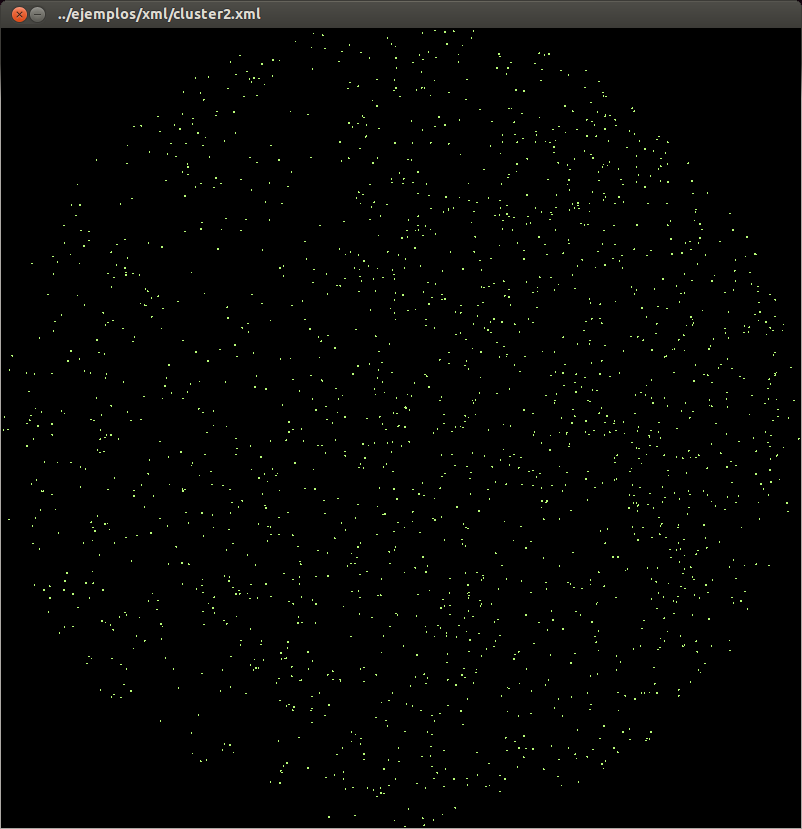
\includegraphics[width=0.5\linewidth]{cluster2-in} 
\label{fig:cluster2-in}}
\subfloat[Salida del \CSUO{}]{
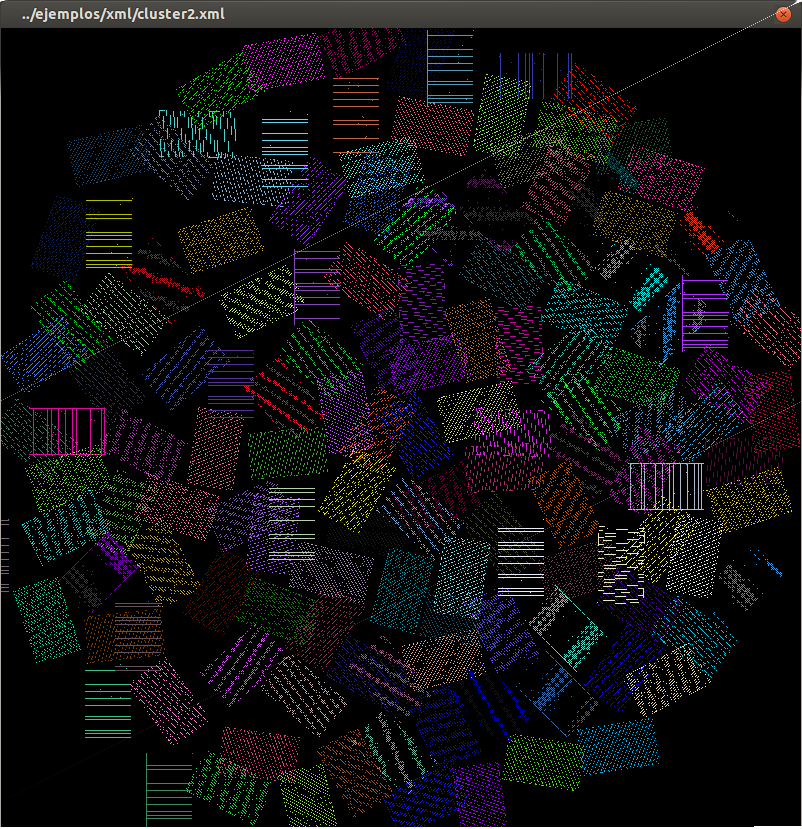
\includegraphics[width=0.5\linewidth]{cluster2-out}
\label{fig:cluster2-out}}
\caption{Ejemplo \texttt{cluster2.xml}. Segundo ejemplo cuyos objetos muestran una distribución concéntrica.}
\end{figure}
%%%%%%%%%%%%%%%%%%%%%%%%%%%%%%%%%%%%%%%%%%%%%%%%%%%%%%%%%%%%%%

\begin{table*}[!ht]
\centering
\begin{tabular}{||l||c|c||}
\hline
\hline
RESULTADOS & Apuntados & Tiempo \\
\hline
\hline
Sin opciones & 138 & 1' 57.42'' \\
\hline
Sin bordes & 152& 2' 1.68'' \\
\hline
Beam Switching & 213 & 2' 19.05'' \\
\hline
Sin bordes + Beam S. & 263 & 4' 19.05'' \\
\hline
\hline
\end{tabular}
\caption{Resultados del ejemplo \texttt{cluster2.xml}}
\end{table*}

Como se observa en los resultados obtenidos, a pesar de que el número de
apuntados necesarios para recoger todos los objetos no es mucho mayor (una
diferencia de 15 apuntados), sí lo es el tiempo que tarda, pasando de
aproximadamente dos minutos a algo más de cuatro minutos y medio. No obstante,
si nos fijamos en el tercer caso, en el que se usa la técnica del beam
switching, vemos que con una diferencia de 33 apuntados, apenas aumenta 1 minuto
el tiempo.

\subsection {Ejemplo: \texttt{cluster3.xml}}
Este ejemplo es igual que los dos anteriores, es decir, tiene una disposición
circular y consta de 1074 objetos. Igual que en el anterior esperábamos tiempos
mayores debido a que era el ejemplo de mayor tamaño, en este esperamos mejores
tiempos al ser el que presenta menor número de elementos.

%%%%%%%%%%%%%%%%%%%% Fig. %%%%%%%%%%%%%%%%%%%%%%%%%%%%%%%%%%%
\begin{figure}[!htb]
\centering
\subfloat[Entrada]{
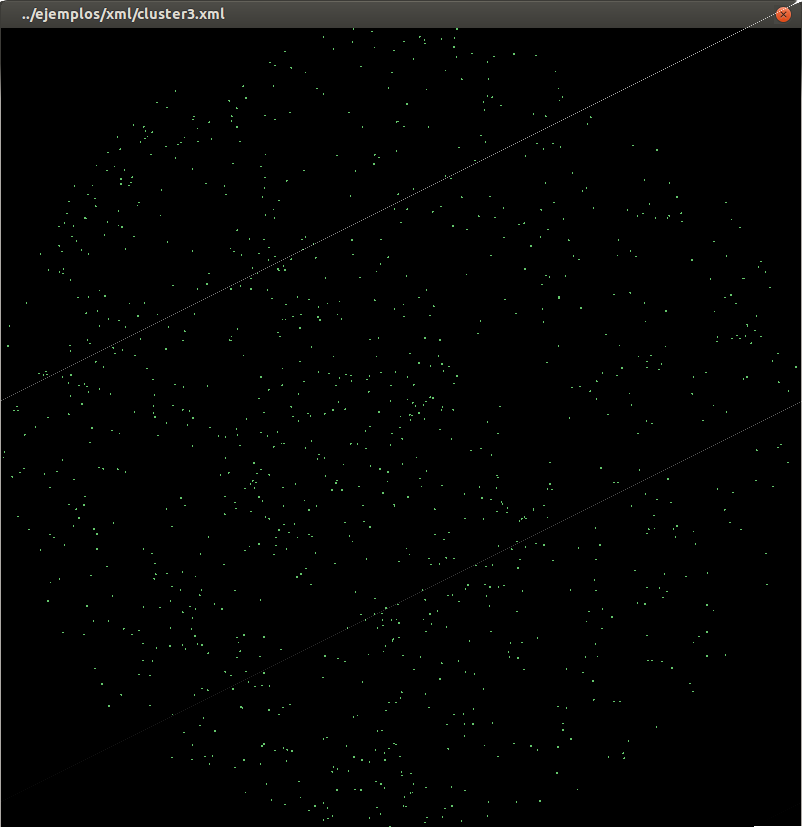
\includegraphics[width=0.5\linewidth]{cluster3-in} 
\label{fig:cluster3-in}}
\subfloat[Salida del \CSUO{}]{
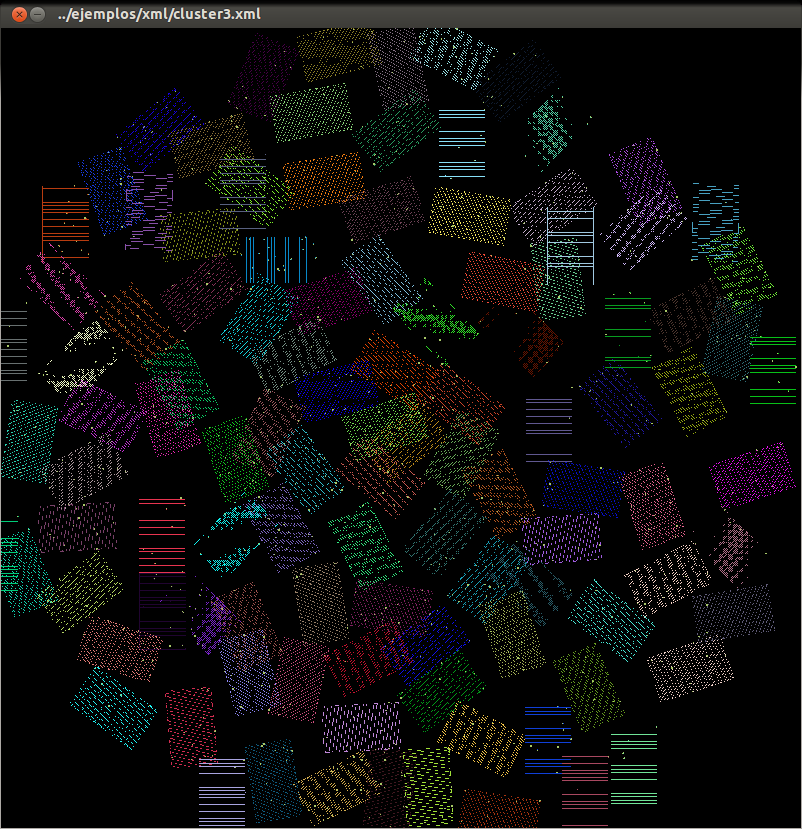
\includegraphics[width=0.5\linewidth]{cluster3-out}
\label{fig:cluster3-out}}
\caption{Ejemplo \texttt{cluster3.xml}. Tercer caso real cuyos objetos muestran una distribución concéntrica.}
\end{figure}
%%%%%%%%%%%%%%%%%%%%%%%%%%%%%%%%%%%%%%%%%%%%%%%%%%%%%%%%%%%%%%

\begin{table*}[!ht]
\centering
\begin{tabular}{||l||c|c||}
\hline
\hline
RESULTADOS & Apuntados & Tiempo \\
\hline
\hline
Sin opciones & 109 & 31.09'' \\
\hline
Sin bordes & 117 & 38.57'' \\
\hline
Beam Switching & 153 & 1' 4.49'' \\
\hline
Sin bordes + Beam S. & 180 & 1' 16.68'' \\
\hline
\hline
\end{tabular}
\caption{Resultados del ejemplo \texttt{cluster3.xml}}
\end{table*}

Los resultados obtenidos son similares a los del primer ejemplo, y no distan
tanto entre sí como los dos primeros a pesar de tener más o menos la misma
diferencia de objetos.
